% -----------------------------------------------------------------------------
\section{Examples}\label{sec:examples}
% -----------------------------------------------------------------------------

This section contains prototypical examples, including use of all
current glyphs to attempt to ensure that their use is clear.

\begin{figure}[h!]
\includegraphics[scale=0.5]{figures/apdx-examples/apdx-exa1.pdf}
\caption{DNA sequence for a functional unit in which the pTet promoter and an anonymous ribosome entry site regulate expression of a coding sequence for GFP, ended by a terminator.}
\label{f:apdx:exa1}
\end{figure}

\begin{figure}[h!]
\includegraphics[scale=0.5]{figures/apdx-examples/apdx-exa2.pdf}
\caption{The same functional unit as in \ref{f:apdx:exa1}, with additional assembly-focused information: there is a 5' overhang before the promoter, a 3' overhand after the terminator, and an assembly scar between the promoter and the ribosome entry site left over from a prior step of assembly.}
\label{f:apdx:exa2}
\end{figure}

\begin{figure}[h!]
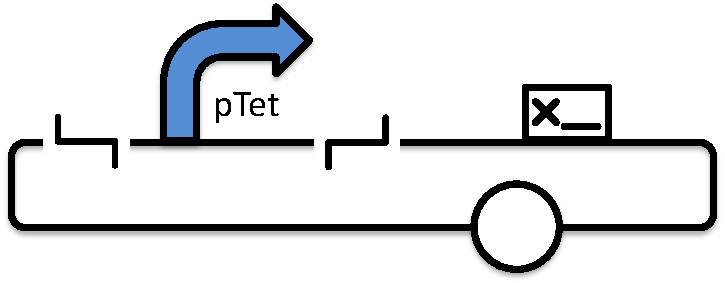
\includegraphics[scale=0.5]{figures/apdx-examples/apdx-exa3.pdf}
\caption{Promoter pTet stored in a circular plasmid. The promoter is prepared for being cut out of the plasmid: it is preceded by a 5' sticky end restriction site and followed by a 3' stick end restriction site.  In addition, the plasmid has been bar-coded with a signature and has its origin of replication marked.}
\label{f:apdx:exa3}
\end{figure}

\begin{figure}[h!]
\includegraphics[scale=0.5]{figures/apdx-examples/apdx-exa4.pdf}
\caption{Promoter stored in a plasmid as in \ref{f:apdx:exa3}, except that the restriction sites before and after the promoter are blunt-end.}
\label{f:apdx:exa4}
\end{figure}

\begin{figure}[h!]
\includegraphics[scale=0.5]{figures/apdx-examples/apdx-exa5.pdf}
\caption{Promoter stored in a plasmid as in \ref{f:apdx:exa3}, except that the cut structure of the restriction sites before and after the promoter is not specified.}
\label{f:apdx:exa5}
\end{figure}

\begin{figure}[h!]
\includegraphics[scale=0.5]{figures/apdx-examples/apdx-exa6.pdf}
\caption{Promoter stored in a plasmid as in \ref{f:apdx:exa3}, except that there is a ribonuclease site after the promoter rather than restriction sites flanking it.}
\label{f:apdx:exa6}
\end{figure}

\begin{figure}[h!]
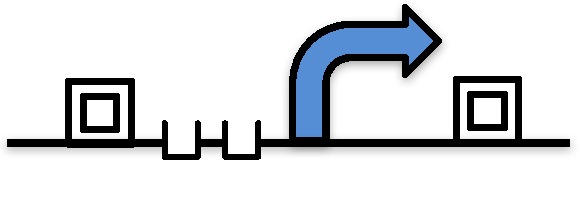
\includegraphics[scale=0.5]{figures/apdx-examples/apdx-exa7.pdf}
\caption{Detailed design of a promoter, in which the transcription start site is preceded by two operator sites where regulators bind.}
\label{f:apdx:exa7}
\end{figure}

\begin{figure}[h!]
\includegraphics[scale=0.5]{figures/apdx-examples/apdx-exa8.pdf}
\caption{Promoter regulating the production of an engineered composite sequence that includes RNA and protein stability elements at its 3' end, as well as an internal site for protease cleavage, as well as the expansion of the composite to show it contains a ribosome entry site. coding sequence, and other omitted details.  Single residue locations of interest are indicated for the DNA (before the promoter), RNA (after the ribosome entry site), and protein (in the CDS).}
\label{f:apdx:exa8}
\end{figure}

\begin{figure}[h!]
\includegraphics[scale=0.5]{figures/apdx-examples/apdx-exa9.pdf}
\caption{DNA sequence with three primer binding sites.}
\label{f:apdx:exa9}
\end{figure}

\begin{figure}[h!]
\includegraphics[scale=0.5]{figures/apdx-examples/apdx-exa10.pdf}
\caption{The same functional unit as in \ref{f:apdx:exa1}, except that information about the CDS is missing, leaving it to fall back on the default unspecified glyph.}
\label{f:apdx:exa10}
\end{figure}

\begin{figure}[h!]
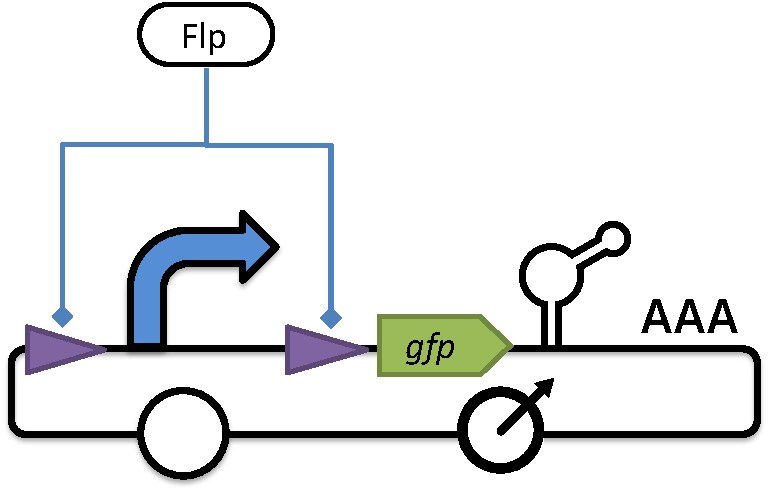
\includegraphics[scale=0.5]{figures/apdx-examples/apdx-exa11.pdf}
\caption{Promoter regulating the expression of GFP, which is also regulated by an aptamer between it and the poly-A tail of the transcript. The promoter can be cut out by a pair of recombinase target sites, which are acted on by the Flp protein.  The whole construct is stored in a circular plasmid with an origin of replication and also an origin of transfer.}
\label{f:apdx:exa11}
\end{figure}

\begin{figure}[h!]
\includegraphics[scale=0.5]{figures/apdx-examples/apdx-exa12.pdf}
\caption{Promoter stimulated by the CDS that it regulates.}
\label{f:apdx:exa12}
\end{figure}

\begin{figure}[h!]
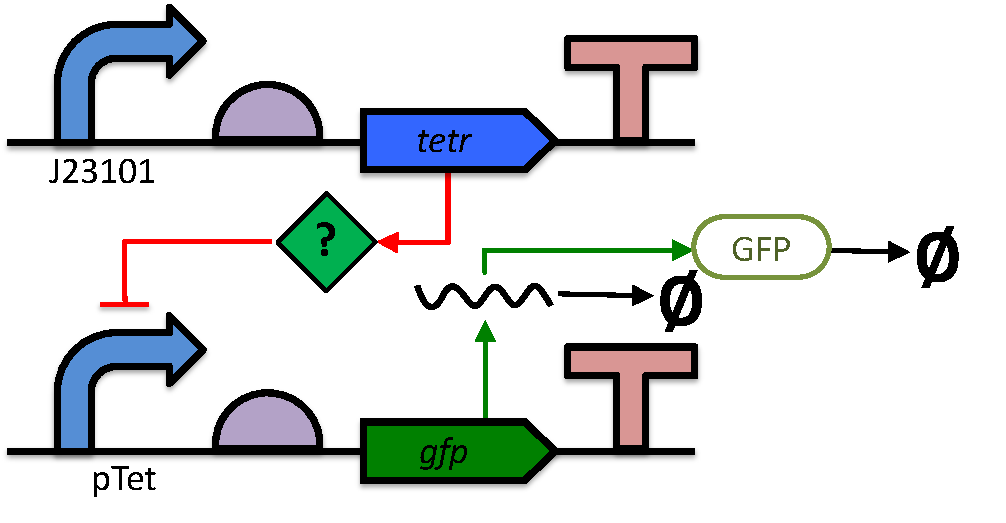
\includegraphics[scale=0.5]{figures/apdx-examples/apdx-exa13.pdf}
\caption{Constitutive production of TetR, except that information about the protein is missing, leaving it as the default unspecified glyph. TetR represses the pTet promoter, which is regulating production of GFP.  The diagram of GFP production explicitly includes the intermediate mRNA and the degradation of both the mRNA and protein products.}
\label{f:apdx:exa13}
\end{figure}

\begin{figure}[h!]
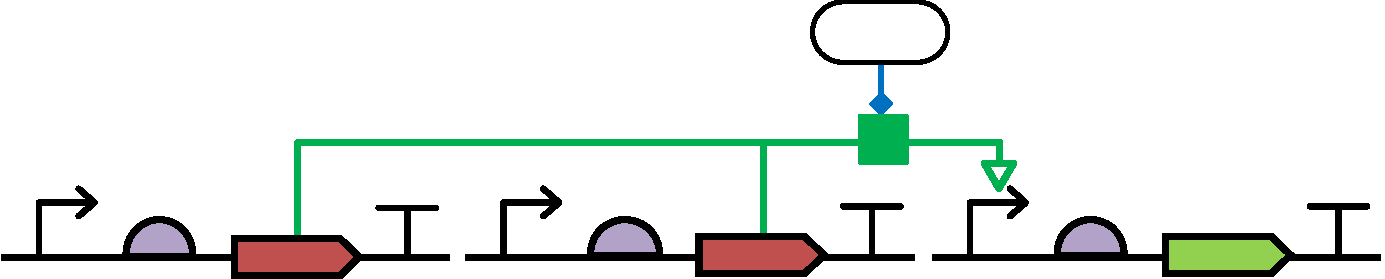
\includegraphics[scale=0.5]{figures/apdx-examples/apdx-exa14.pdf}
\caption{Phosphorylation of an inactive transcription factor (produced by two different CDSs) by a kinase to form an active transcriptional activator, which then stimulates a promoter.}
\label{f:apdx:exa14}
\end{figure}

\begin{figure}[h!]
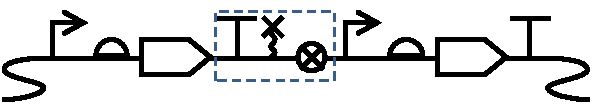
\includegraphics[scale=0.5]{figures/apdx-examples/apdx-exa15.pdf}
\caption{Ribozyme and spacer between two transcriptional units, forming a separation module with the preceding terminator (dashed box), with the whole construct integrated into the chromosome.}
\label{f:apdx:exa15}
\end{figure}

\begin{figure}[h!]
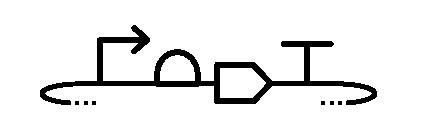
\includegraphics[scale=1.0]{figures/apdx-examples/apdx-exa16-circular-plasmid-example.pdf}
\caption{A circular plasmid containing a functional unit consisting of promoter, ribosome entry site, CDS, and terminator.}\label{f:apdx:exa16}
\end{figure}

\begin{figure}[h!]
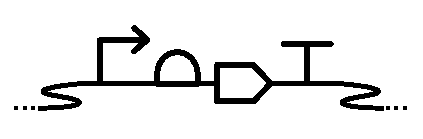
\includegraphics[scale=1.0]{figures/apdx-examples/apdx-exa17-chromosomal-locus-example.pdf}
\caption{A functional unit consisting of promoter, ribosome entry site, CDS, and terminator, all integrated together into the chromosome.}
\label{f:apdx:exa17}
\end{figure}

\begin{figure}[h!]
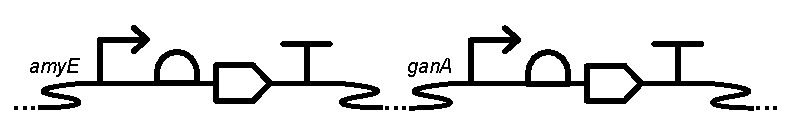
\includegraphics[scale=1.0]{figures/apdx-examples/apdx-exa18-chromosomal-locus-example2.pdf}
\caption{Two functional units, one integrated into the amyE locus, another integrated into the ganA locus}\label{f:apdx:exa18}
\end{figure}

\begin{figure}[h!]
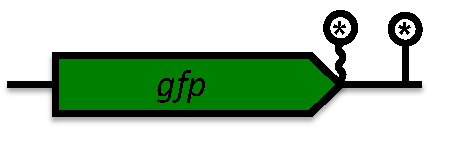
\includegraphics[scale=0.5]{figures/apdx-examples/apdx-exa19-stop-sites.pdf}
\caption{Coding sequence marking the stop codon at its end and transcriptional end site farther down the sequence.}
\label{f:apdx:exa19}
\end{figure}

\begin{figure}[h!]
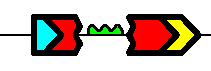
\includegraphics[scale=1.0]{figures/apdx-examples/apdx-exa20-intron.pdf}
\caption{A coding sequence with three domains: an N-tag (blue), C-tag (yellow), and internal region (red) interrupted by an intron that includes a gRNA non-coding RNA sequence (green).}
\label{f:apdx:exa20}
\end{figure}

\begin{figure}[h!]
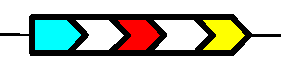
\includegraphics[scale=1.0]{figures/apdx-examples/apdx-exa21-polypeptide-region.pdf}
\caption{A coding sequence with three designated domains, an N-tag (blue), C-tag (yellow), and internal region (red).}
\label{f:apdx:exa21}
\end{figure}

\begin{figure}[h!]
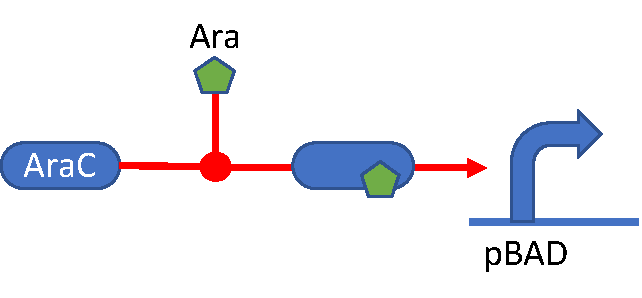
\includegraphics[scale=0.75]{figures/apdx-examples/apdx-exa22.pdf}
\caption{The AraC protein and arabinose associating into a complex that activates the pBAD promoter.}
\label{f:apdx:exa22}
\end{figure}

\begin{figure}[h!]
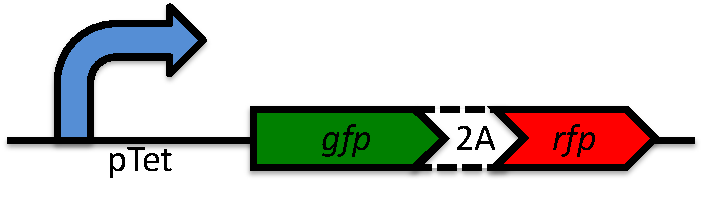
\includegraphics[scale=0.75]{figures/apdx-examples/apdx-exa23-bicistronic.pdf}
\caption{Bicistronic expression of both GFP and RFP from a signal coding sequence, by means of a 2A self-cleaving polypeptide region.}
\label{f:apdx:exa23}
\end{figure}



% Figure black magic: adjust the size here as needed to get the spacing on the last page of the section correct.
%\begin{figure}[h!]
%\vspace{2in}
%\end{figure}


